\documentclass[border=0pt]{standalone}
\usepackage{tikz}
\usepackage{amsmath, amsthm, amssymb}
%\input{commondefinitions}
\usetikzlibrary{plotmarks}
\newcommand\marksymbol[2]{\tikz[#2,scale=1.2]\pgfuseplotmark{#1};}

\colorlet{coscolor}{blue}
\newcommand{\cuadritotikz}{
% \pgfmathsetmacro{\unitstep}{5.2}
% \node at (-0.5,0.5) {(a)} ;
    \foreach \x in {0,1,2,3} {
      \foreach \y in {0,1,2,3} {
        \begin{scope}[shift={(\x,-\y)}] 
          \draw[black!10] (0,0) rectangle (1,1); 
%           \node at (0.5,0.5) {$\tau_{\y,\x}$};
         \end{scope}
%         \node[block] at (2,-\y) (block\y) {$f_\y$};
%         \draw[->] (block\y.east) -- +(0.5,0);
    }
    }
 \draw (0,-3) rectangle (4,1);
}

\begin{document}
\pagestyle{empty}
\begin{tikzpicture}[x=0.47cm, y=0.47cm] % {{{
\pgfmathsetmacro{\unitstep}{3.35}
% Coordenadas   {{{
\node at (-0.6,0.5) {(a)} ;
\draw[black!10] (0,0) rectangle (1,1); \node at (0.5,0.5) {$\tau_0$} ;
\begin{scope}[shift={(0,-1)}]
\draw[black!10] (0,0) rectangle (1,1); \node at (0.5,0.5) {$\tau_1$} ;
\end{scope}
\begin{scope}[shift={(0,-2)}]
\draw[black!10] (0,0) rectangle (1,1); \node at (0.5,0.5) {$\tau_2$} ;
\end{scope}
\begin{scope}[shift={(0,-3)}]
\draw[black!10] (0,0) rectangle (1,1); \node at (0.5,0.5) {$\tau_3$} ;
\end{scope} 
\draw (0,-3) rectangle (1,1); 
% }}}
\begin{scope}[shift={(1*\unitstep,0)}] % Identity {{{
% \begin{scope}[shift={(\unitstep*2,0)}]
\node at (-0.6,0.5) {(b)} ;
\fill[black] (0,0) rectangle (1,1);
\draw[black!10] (0,0) rectangle (1,1);
\begin{scope}[shift={(0,-1)}] \draw[black!10] (0,0) rectangle (1,1); \end{scope}
\begin{scope}[shift={(0,-2)}] \draw[black!10] (0,0) rectangle (1,1); \end{scope}
\begin{scope}[shift={(0,-3)}] \draw[black!10] (0,0) rectangle (1,1); \end{scope}
\draw (0,-3) rectangle (1,1); 
\begin{scope}[shift={(0,-1)}] \fill[black] (0,0) rectangle (1,1); \end{scope}
\begin{scope}[shift={(0,-2)}] \fill[black] (0,0) rectangle (1,1); \end{scope}
\begin{scope}[shift={(0,-3)}] \fill[black] (0,0) rectangle (1,1); \end{scope}
\end{scope} % }}}
\begin{scope}[shift={(2*\unitstep,0)}] % Dephasing {{{
\node at (-0.6,0.5) {(c)} ;
\fill[black] (0,0) rectangle (1,1);
% \draw (0,0) rectangle (1,1);
\draw[black!10] (0,0) rectangle (1,1);
\begin{scope}[shift={(0,-1)}] \draw[black!10] (0,0) rectangle (1,1); \end{scope}
\begin{scope}[shift={(0,-2)}] \draw[black!10] (0,0) rectangle (1,1); \end{scope}
\begin{scope}[shift={(0,-3)}] \draw[black!10] (0,0) rectangle (1,1); \end{scope}
\draw (0,-3) rectangle (1,1); 
% \begin{scope}[shift={(0,-1)}] \fill[black] (0,0) rectangle (1,1); \end{scope}
% \begin{scope}[shift={(0,-1)}] \draw (0,0) rectangle (1,1); \end{scope}
% \begin{scope}[shift={(0,-2)}] \fill[black] (0,0) rectangle (1,1); \end{scope}
% \begin{scope}[shift={(0,-2)}] \draw (0,0) rectangle (1,1); \end{scope}
\begin{scope}[shift={(0,-3)}] \fill[black] (0,0) rectangle (1,1); \end{scope}
% \begin{scope}[shift={(0,-3)}] \draw (0,0) rectangle (1,1); \end{scope}
\end{scope} % }}}
\begin{scope}[shift={(3*\unitstep,0)}] % Depolarization {{{
\node at (-0.6,0.5) {(d)} ;
\fill[black] (0,0) rectangle (1,1);
% \draw (0,0) rectangle (1,1);
\draw[black!10] (0,0) rectangle (1,1);
\begin{scope}[shift={(0,-1)}] \draw[black!10] (0,0) rectangle (1,1); \end{scope}
\begin{scope}[shift={(0,-2)}] \draw[black!10] (0,0) rectangle (1,1); \end{scope}
\begin{scope}[shift={(0,-3)}] \draw[black!10] (0,0) rectangle (1,1); \end{scope}
\draw (0,-3) rectangle (1,1); 
% \begin{scope}[shift={(0,-1)}] \fill[black] (0,0) rectangle (1,1); \end{scope}
% \begin{scope}[shift={(0,-1)}] \draw (0,0) rectangle (1,1); \end{scope}
% \begin{scope}[shift={(0,-2)}] \fill[black] (0,0) rectangle (1,1); \end{scope}
% \begin{scope}[shift={(0,-2)}] \draw (0,0) rectangle (1,1); \end{scope}
% \begin{scope}[shift={(0,-3)}] \fill[black] (0,0) rectangle (1,1); \end{scope}
% \begin{scope}[shift={(0,-3)}] \draw (0,0) rectangle (1,1); \end{scope}
\end{scope} % }}}
\begin{scope}[shift={(4*\unitstep,0)}] % (e) canal malo {{{
\node at (-0.6,0.5) {(e)} ;
\fill[black] (0,0) rectangle (1,1);
% \draw (0,0) rectangle (1,1);
\draw[black!10] (0,0) rectangle (1,1);
\begin{scope}[shift={(0,-1)}] \draw[black!10] (0,0) rectangle (1,1); \end{scope}
\begin{scope}[shift={(0,-2)}] \draw[black!10] (0,0) rectangle (1,1); \end{scope}
\begin{scope}[shift={(0,-3)}] \draw[black!10] (0,0) rectangle (1,1); \end{scope}
% \begin{scope}[shift={(0,-1)}] \fill[black] (0,0) rectangle (1,1); \end{scope}
% \begin{scope}[shift={(0,-1)}] \draw (0,0) rectangle (1,1); \end{scope}
\begin{scope}[shift={(0,-2)}] \fill[black] (0,0) rectangle (1,1); \end{scope}
% \begin{scope}[shift={(0,-2)}] \draw (0,0) rectangle (1,1); \end{scope}
\begin{scope}[shift={(0,-1)}] \fill[black] (0,0) rectangle (1,1); \end{scope}
% \begin{scope}[shift={(0,-3)}] \draw (0,0) rectangle (1,1); \end{scope}
\draw (0,-3) rectangle (1,1);
\end{scope}\\[10ex] % }}}
%\end{tikzpicture} % }}}
% \begin{tikzpicture} 
%     \node at (0,  0)  {\includegraphics{distribution_eigenvalues}};
%     \node at (0,-2.6) {\footnotesize $\lambda$};
%     \node at (-1.4,-.02) {\footnotesize Re$\lambda$};
%     \node at (-3.5,1.5) {\rotatebox{90}{\footnotesize Im$\lambda$}};
% %     \node at (0,-2.4) {$\eta$};
%   \node[rotate=90] at (-4.3,0.0) {\footnotesize probability density};
% %   \node[rotate=90] at (-3.35,-1.6) {$\widetilde{Z}_Q^{\textbf{P}}$};
% \node[anchor=west] at (-3.5,-.38) {\footnotesize \marksymbol{square*}{blue} Random Channel};
% \node[anchor=west] at (-3.5,-.72) {\footnotesize \marksymbol{square*}{red} Two body};
% \node[anchor=west] at (-3.5,-1) {\footnotesize \marksymbol{square*}{green} Chain};
% % \node[anchor=west] at (-2.45,1.7) {\tiny \marksymbol{square*}{black!45!green} Chain};
% %   \node[anchor=west] at (-2.45,1.45) {\tiny \marksymbol{triangle*}{magenta} RSM $n_{\text{ens}}=1000$};
% %   \node[anchor=west] at (-2.45,1.2) {\tiny \marksymbol{*}{black!50!green!10!cyan} RESM $n_{\text{ens}}=1$};
% %   \node[anchor=west] at (-2.45,0.95) {\tiny \marksymbol{diamond*}{red} RESM $n_{\text{ens}}=10$};
% %   \node[anchor=west] at (-2.45,0.70) {\tiny \hspace{.2cm} $\widetilde{Z}_Q^{\textbf{P}}$};
% %   \node[anchor=west] at (-3, 2.5) {$(a)$};
% %   \node[rotate=90] at (-3.35,-0.3) {RESM-10,};
% %   \node[rotate=90] at (-3.35,1.4) {RESM-1};
% %   \node[rotate=90] at (2.8,-0.55) {RSM-1000,};
% %   \node[rotate=90] at (2.8,1.15) {RSM-10};
% %   \node[rotate=90] at (-3.35, -1.2) {\marksymbol{diamond*}{red}};
% %   \node at (-3.35, 0.65) {\marksymbol{*}{black!50!green!10!cyan}};
% %   \node[rotate=90] at (2.8, -1.5) {\marksymbol{triangle*}{magenta}};
% %   \node at (2.8, 0.4) {\marksymbol{square*}{black!45!green}};
% %    \begin{scope}
% %        \filldraw[thick,blue] (-2.35,0.70) -- (-2.35+0.2,0.70);
% %    \end{scope}
% \end{tikzpicture} 
%\newline
%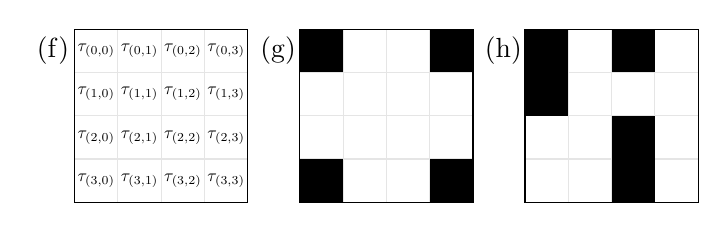
\begin{tikzpicture}[x=0.55cm, y=0.55cm] % {{{
\pgfmathsetmacro{\unitstep}{5.2}
\begin{scope}[shift={(0*\unitstep,-0.85*\unitstep)}] % Coordenadas {{{
\node at (-0.5,0.5) {(f)} ;
% \cuadritotikz{}
    \foreach \x in {0,1,2,3} {
      \foreach \y in {0,1,2,3} {
        \begin{scope}[shift={(\x,-\y)}] 
          \draw[black!10] (0,0) rectangle (1,1); 
%           \draw (0,0) rectangle (1,1); 
          \node at (0.5,0.5) {\scalebox{.63}{$\tau_{(\y,\x)}$}};
         \end{scope}
%         \node at (0,-\y) (input\y) {$i_\y$};
%         \node[block] at (2,-\y) (block\y) {$f_\y$};
%         \draw[->] (input\y) -- (block\y);
%         \draw[->] (block\y.east) -- +(0.5,0);
    }
    }
 \draw (0,-3) rectangle (4,1);
\end{scope} % }}}
\begin{scope}[shift={(1*\unitstep,-0.85*\unitstep)}] % Good channel {{{
\node at (-0.5,0.5) {(g)} ;
\cuadritotikz{}
%     \foreach \x in {0,1,2,3} {
%       \foreach \y in {0,1,2,3} {
%         \begin{scope}[shift={(\x,-\y)}] 
%           \draw (0,0) rectangle (1,1); 
% %           \node at (0.5,0.5) {$\tau_{\y,\x}$};
%          \end{scope}
% %         \node at (0,-\y) (input\y) {$i_\y$};
% %         \node[block] at (2,-\y) (block\y) {$f_\y$};
% %         \draw[->] (input\y) -- (block\y);
% %         \draw[->] (block\y.east) -- +(0.5,0);
%     }
%     }
\begin{scope}[shift={(0,-3)}] \fill[black] (0,0) rectangle (1,1); \end{scope}
\begin{scope}[shift={(3,-3)}] \fill[black] (0,0) rectangle (1,1); \end{scope}
\begin{scope}[shift={(0,0)}] \fill[black] (0,0) rectangle (1,1); \end{scope}
\begin{scope}[shift={(3,0)}] \fill[black] (0,0) rectangle (1,1); \end{scope}
\end{scope} % }}}
\begin{scope}[shift={(2*\unitstep,-0.85*\unitstep)}] % Good channel {{{
\node at (-0.5,0.5) {(h)} ;
\cuadritotikz{}
%     \foreach \x in {0,1,2,3} {
%       \foreach \y in {0,1,2,3} {
%         \begin{scope}[shift={(\x,-\y)}] 
%           \draw (0,0) rectangle (1,1); 
% %           \node at (0.5,0.5) {$\tau_{\y,\x}$};
%          \end{scope}
% %         \node at (0,-\y) (input\y) {$i_\y$};
% %         \node[block] at (2,-\y) (block\y) {$f_\y$};
% %         \draw[->] (input\y) -- (block\y);
% %         \draw[->] (block\y.east) -- +(0.5,0);
%     }
%     }
\begin{scope}[shift={(0,0)}] \fill[black] (0,0) rectangle (1,1); \end{scope}
\begin{scope}[shift={(0,-1)}] \fill[black] (0,0) rectangle (1,1); \end{scope}
\begin{scope}[shift={(2,0)}] \fill[black] (0,0) rectangle (1,1); \end{scope}
\begin{scope}[shift={(2,-2)}] \fill[black] (0,0) rectangle (1,1); \end{scope}
\begin{scope}[shift={(2,-3)}] \fill[black] (0,0) rectangle (1,1); \end{scope}
\end{scope} % }}}
\end{tikzpicture} % }}}
\end{document}
